%//==============================--@--==============================//%
\subsection[2.1 Resposta no Tempo]{\hspace*{0.075 em}\raisebox{0.2 em}{$\pmb{\drsh}$} Resposta no Tempo}
\label{sec:resposta-no-tempo}

\begin{theo}[\underline{Def.:} Função de transferência]{def:ft}\label{def:ft}
    \noindent ``The transfer function can be formally defined as follows: The function, which is the transfer gain from $U(s)$ to $Y(s)$ --- input to output --- is called the transfer
    function of the system. It is the ratio of the Laplace transform of the output of the
    system to the Laplace transform of the input.

    $$
        \dfrac{Y(s)}{U(s)} = F(s)
    $$
    \noindent with the key assumption that all of the initial conditions on the system are zero."\cite{FranklinPowell2015}
\end{theo}

\noindent A função de transferência é um conceito potente:

\begin{itemize}
    \item não depende nem da entrada nem da saída do sistema
    \item caracteriza completamente o sistema do ponto de vista de entrada-saída
\end{itemize}

$$
     F(s) = \dfrac{Y(s)}{U(s)} = \dfrac{\text{polinómio de grau m}}{\text{polinómio de grau n}}
$$

\begin{itemize}
    \item n > m a função de transferência diz-se estritamente própria
    \item n $\ge$ m a função de transferência diz-se prória
    \item n < m a função de transferência diz-se imprópria
\end{itemize}

\noindent ``The roots of the denominator $U(s)$, $\{p_1,p_2,\dots,p_n\}$, are called the poles of the system.
The poles are locations in the s-plane where the magnitude of the transfer function becomes infinite if $s = p_i$:

$$
    \boxed{|F(s)|_{s = p_i} = \infty}
$$

\noindent The roots of the numerator, $Y(s)$, $\{z_1,z_2, \dots, z_n\}$ are called the finite zeros of the system. The zeros are locations in the s-plane where the transfer function is zero. If $s = z_i$:"\cite{FranklinPowell2015}

$$
    \boxed{|F(s)|_{s = z_i} = 0}
$$

\noindent A sua interação influência a característica da resposta do sistema:

{\setlength{\tabcolsep}{16pt}
\begin{center}
    \begin{tabular}{p{0.4\textwidth} | p{0.4\textwidth}}
        \centerline{\underline{$\#\textbf{pólos} > \#\textbf{zeros}$}} & \centerline{\underline{$\#\textbf{pólos} > \#\textbf{zeros}+1$}} \\[-14pt]
        Resposta ao escalão contínua & Derivada da resposta contínua \\[4pt]
        \centerline{\underline{$\#\textbf{pólos} = \#\textbf{zeros}$}} & \centerline{\underline{$\#\textbf{pólos} = \#\textbf{zeros}+1$}} \\[-14pt]
        Resposta descontínua, com salto finito & Derivada da resposta descontínua, mas finita \\[4pt]
        \centerline{\underline{$\#\textbf{pólos} < \#\textbf{zeros}$}} & \centerline{\underline{$\#\textbf{pólos} < \#\textbf{zeros}+1$}} \\[-14pt]
        Resposta descontínua, com salto infinito & Derivada da resposta descont.,  infinita \\
        \bottomrule
    \end{tabular}
\end{center}
}

\newpage
\subsubsection[2.1.1 Análise da função de transferência]{$\pmb{\rightarrow}$ Análise da função de transferência}

Se $f(t)$ não contiver impulsos ou singularidades de ordem superior na origem e convergir para um valor constante quando $t \to +\infty$, então, aplicam-se os teoremas:
\begin{center}%
    \begin{tabular}{c c}%
        \begin{minipage}{0.425\linewidth}%
            \begin{theo}[\underline{Teorema do Valor Incial}]{teo:inicial-value}\label{teo:inicial-value}
                $$
                    \lim_{t \to 0} f(t) = \lim_{s \to +\infty} sF(s)
                $$
            \end{theo}%
        \end{minipage}%
        &%
        \begin{minipage}{0.425\linewidth}%
            \begin{theo}[\underline{Teorema do Valor Final}]{teo:final-value}\label{teo:final-value}
                $$
                    \lim_{t \to +\infty} f(t) = \lim_{s \to 0} sF(s)
                $$
            \end{theo}%
        \end{minipage}%
    \end{tabular}%
\end{center}%

\subsubsection[2.1.2 Resposta ao escalão unitário de sistemas LIT]{$\pmb{\rightarrow}$ Resposta ao escalão unitário de sistemas LIT}

\begin{figure}[H]
    \centering
    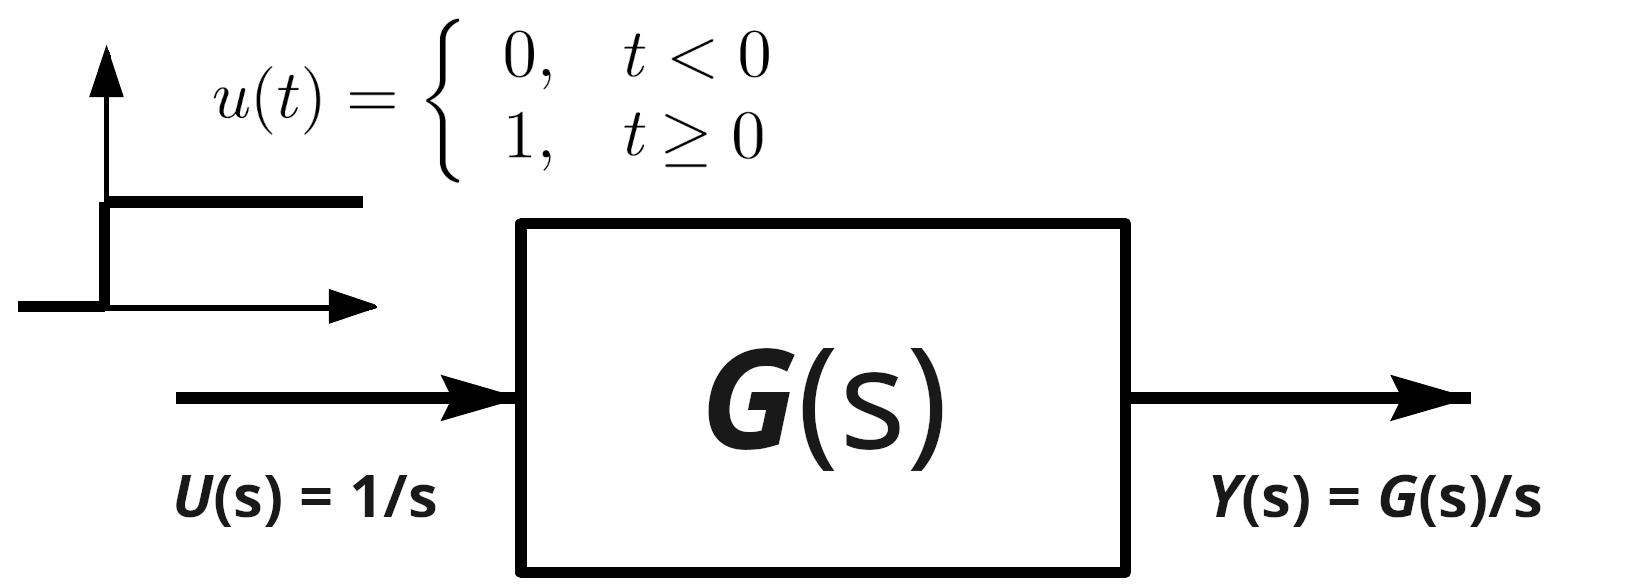
\includegraphics[width = 0.5\linewidth]{img/2/unit-step-response.png}
    \caption{Resposta do sistema ao degrau unitário.}
    \label{fig:unit-step-response}
\end{figure}

{
\mdfsetup{linewidth=2pt}

\begin{mdframed}
    \begin{itemize}
    \item[$\blacktriangle$] \underline{Valor final da resposta} ao escalão unitário:
        
        \vspace{-1em}
        $$
            \lim_{t \to +\infty} y(t) = \lim_{s \to 0} sY(s) = \lim_{s \to 0} s\frac{G(s)}{s} = G(0)
        $$
        
    \vspace{-0.5em}
    \item[$\blacktriangle$] \underline{Valor inicial da resposta} ao escalão:
        
        \vspace{-1em}
        $$
            \lim_{t \to 0} y(t) = \lim_{s \to +\infty} sY(s) = \lim_{s \to +\infty} s\frac{G(s)}{s} = \lim_{s \to +\infty} G(s)
        $$
        
    \vspace{-0.5em}
    \item[$\blacktriangle$] \underline{Valor inicial da derivada da resposta} ao escalão unitário:
        
        \vspace{-1em}
        $$
            \lim_{t \to 0} \dot{y}(t) = \lim_{s \to +\infty} s\, (sY(s)) = \lim_{s \to +\infty} s^2\frac{G(s)}{s} = \lim_{s \to +\infty} sG(s)
        $$

    \vspace{-0.5em}
    \item[$\blacktriangle$] \underline{Valor final da derivada da resposta} ao escalão unitário:
        
        \vspace{-1em}
        $$
            \lim_{t \to +\infty} \dot{y}(t) = \lim_{s \to 0} s\, (sY(s)) = \lim_{s \to 0} s^2\frac{G(s)}{s} = \lim_{s \to 0} s G(s)
        $$
    \end{itemize}
\end{mdframed}
}
\paragraph[2.1.2.1 Sistema de 1º ordem]{$\pmb{\star}$ Sistema de 1º ordem:} Seja $G(s)$ a função de transferência de um sistema de primeira ordem em resposta ao escalão unitário:
$$
    G(s) = K_0 \cdot \dfrac{a}{s + a} 
$$
\noindent \textbf{Ganho estático}: O ganho estático, $K_0 = G(0)$, denomina o rácio da relação entre entrada e saída do sistema, na análise \textit{steady state}. 

\vspace{1 em}
\noindent \textbf{Tempo de estabelecimento:} Tempo ao fim do qual a resposta se confina a uma faixa de $\pm x\%,\;\, x \in \{2,3,5,7,\dots\}$
\begin{align*}
    Y(s) &= G(s)U(s)\;\; \overset{\mathcal{L}}{\Longrightarrow}\;\; K_0 (1 - e^{-at}),\;\, t \ge 0\\[4pt]
    t_s &= \dfrac{-\ln(0.02)}{a} \simeq \dfrac{4}{a} = 4\tau
\end{align*}

\noindent Onde $\tau = \frac{1}{a}$ é a constante de tempo do sistema, que denota o tempo necessário para que a resposta ao grau unitário atinga 63\% do seu valor final.

\paragraph[2.1.2.2 Sistema de 2º ordem]{$\pmb{\star}$ Sistema de 2º ordem:} Seja $G(s)$ a função de transferência de um sistema de segunda ordem em resposta ao escalão unitário:
$$
    G(s) = \dfrac{w_n^2}{s^2 + \zeta w_n s + w_n^2} 
$$

\begin{mdframed}
\noindent A resposta do sistema ao degrau unitário está totalmente dependente da localização dos pólos:
$$
    s^2 + \zeta w_n s + w_n^2\;\; \Longrightarrow\;\; s = -\zeta w_n \pm w_n\sqrt{\zeta^2 - 1}
$$

\begin{itemize}
    \item \textbf{Sistema subamortecido:} $0 \ge \zeta < 1$
    $$
        \boxed{s = -\zeta w_n \pm j w_n\sqrt{1 - \zeta^2}}
    $$
    \item \textbf{Sistema criticamente amortecido:} $\zeta = 1$
    $$
        \boxed{s = -w_n}
    $$
    \item \textbf{Sistema sobreamortecido:} $\zeta > 1$
    $$
        \boxed{s = -\zeta w_n \pm w_n\sqrt{\zeta^2 - 1}}
    $$
\end{itemize}

\noindent \textbf{Nota:} Os parâmetros acima mencionados possuem a seguinte nomenclatura:

\begin{itemize}
    \item Frequência das oscilações naturais sem amortecimento, $w_n$
    \item Coeficiente de amortecimento, $\zeta$
    \item Frequência das oscilações amortecidas, $w_d = w_n\sqrt{\zeta^2 - 1}$
\end{itemize}
\end{mdframed}

\vspace{-2em}
\begin{figure}[H]
    \centering
    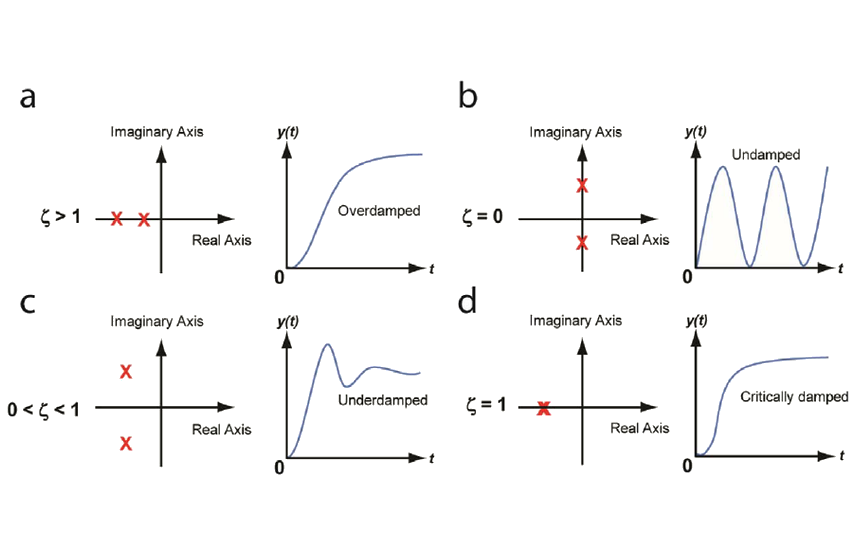
\includegraphics[width = 0.8\linewidth]{img/2/second-order-system.png}
    \caption{Tipos de respostas de sistemas de segunda ordem sem zeros}
    \label{fig:LABEL}
\end{figure}

%//==============================--@--==============================//%
\subsubsection[2.1.3 Especificações do domínio do tempo]{$\pmb{\rightarrow}$ Especificações do domínio do tempo}

\noindent As especificações de desempenho para um projeto de sistema de controle frequentemente envolvem certos requisitos associados à resposta do tempo do sistema. Os requisitos para uma resposta ao degrau unitário são expressos em termos das quantidades padrão:

\begin{itemize}
    \item \textbf{Tempo de crescimento}, \textit{rise time}, $t_r$ tempo que o sistema leva para atingir a proximidade do seu novo ponto de ajuste.
    \item \textbf{Tempo de pico}, \textit{peak time}, $t_p$ é o tempo que o sistema leva a atingir o ponto máximo de sobreelevação.
    \item \textbf{Tempo de estabelecimento}, \textit{setting time}, $t_s$ é o tempo que o sistema leva para transitar para o regime estacionário.
    \item \textbf{Sobreelevação}, \textit{overshoot}, $M_p$ é a quantidade máxima que o sistema ultrapassa o seu valor final, dividido pelo seu valor final (usualmente expresso em percentagem)
\end{itemize}

\paragraph[2.1.3.1 Rise time]{$\pmb{\star}$ Rise time}\mbox{}

\noindent Par um sistema de segunda ordem se zeros, o  \textit{rise time} é dado por:
$$
\boxed{t_r = \dfrac{1.8}{w_n}}
$$
\noindent ``It is accurate only for a second-order system with no zeros; for all other systems, it is a rough approximation to the relationship between $t_r$ and $w_n$."\cite{FranklinPowell2015}

\paragraph[2.1.3.2 Tempo de pico]{$\pmb{\star}$ Tempo de pico}\mbox{}\\

\noindent O tempo de pico é obtido quando se anula a derivada da resposta no tempo do sistema ao grau unitário. Tomando o modelo de segunda ordem sem zeros já acima mencionado:

$$
    y(t) = 1 - e^{-\sigma t}\left(cos w_d t + \dfrac{\sigma}{w_d}\sin w_d t\right),\;\, \sigma = \zeta w_n
$$

A equação acima pode ser reescrita recorrendo à seguinte entidade trigonomérica:
$$
    A\sin(\alpha) + Bcos(\alpha) = C\cos(\alpha - \beta)
$$

\noindent O que resulta na seguinte forma compacta:
$$
    y(t) = 1 - \dfrac{e^{\sigma t}}{\sqrt{1 - \zeta}}\left(\cos{w_d t - \beta}\right)
$$

\noindent A respetiva derivada possui a seguinte forma:
$$
    \dot{y}(t) = e^{-\sigma t}\left(\dfrac{\sigma^2}{w_d} + w_d\right)\sin{w_d t}
$$

\noindent A derivada anula-se para:
$$
    w_d t_p = \pi
$$

\noindent Logo, podemos definir o tempo de pico como:
$$
    \boxed{t_p = \dfrac{\pi}{w_d}}
$$

\paragraph[2.1.3.4 Sobreelevação]{$\pmb{\star}$ Sobreelevação}\mbox{}\\

\noindent A sobreelevação é obtida através da aplicação do resultado previamente obtido na expressão de $y(t)$.
$$
    \boxed{\dfrac{y_{\textit{máx}} - y_{min}}{y_{final}} = M_p = e^{-\pi \zeta / \sqrt{1 - \zeta^2}}}
$$

\paragraph[2.1.3.3 Tempo de estabelecimento]{$\pmb{\star}$ Tempo de estabelecimento}\mbox{}\\

\noindent O tempo de estabelecimento, como já explicictado no sistema de 1ª ordem, é o instante de tempo em que a saída atinge e se mantém numa faixa de $\pm 2\%$ do valor final:

$$
    y(t) = 1 - e^{-\sigma t}\left(cos w_d t + \dfrac{\sigma}{w_d}\sin w_d t\right),\;\, \sigma = \zeta w_n
$$

\noindent ``As an analytic computation, we notice that the deviation of from 1 is the product of the decaying exponential, $e^{-\sigma t}$, and the circular functions sine and cosine. The duration of this error is essentially decided by the transient exponential, so we can define the settling time as
that value of $t_s$ when the decaying exponential reaches $1\%$ (or any other number for that matter, tipically we use $2\%, 5\%, 7\%, \dots$):

$$
    \begin{aligned}
        &e^{\sigma t_s} = 0.01\\
        &t_s = \dfrac{\ln{0.01}}{\sigma} \simeq \dfrac{4.6}{\sigma}
    \end{aligned}
$$

\begin{center}
    \begin{minipage}{0.45\textwidth}
        \begin{itemize}[leftmargin=*]
        \item[] \textbf{\emph{Coeficiente de amortecimento}}: O coeficiente é constante em cada uma das retas apresentadas. Quanto maior for o coeficiente, menor é o \textit{overshoot}.
        \end{itemize}
    \end{minipage}%
    \hfill
    \begin{minipage}{0.55\textwidth}
        \begin{center}
            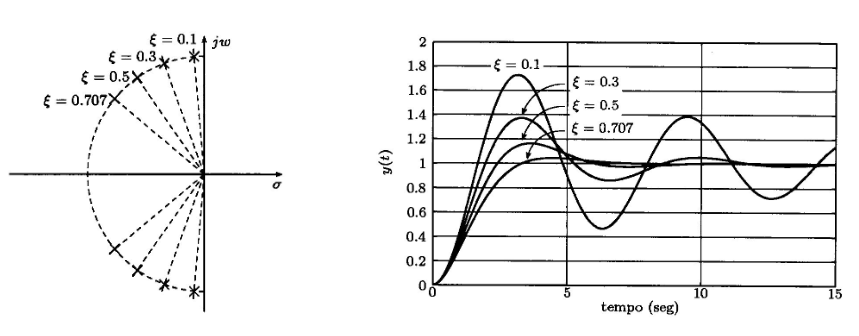
\includegraphics[width=0.95\textwidth]{img/2/overshoot.png}
            \label{img:overshoot}
        \end{center}
    \end{minipage}
\end{center}

\begin{center}
    \begin{minipage}{0.45\textwidth}
        \begin{itemize}[leftmargin=*]
        \item[] \textbf{\emph{Oscilações amortecidas}}: O pa- râmetro $\sigma$ é constante na continuidade da reta apresentada. Quanto maior for $w_d$, menor é o \textit{peak time}.
        \end{itemize}
    \end{minipage}%
    \hfill
    \begin{minipage}{0.55\textwidth}
        \begin{center}
            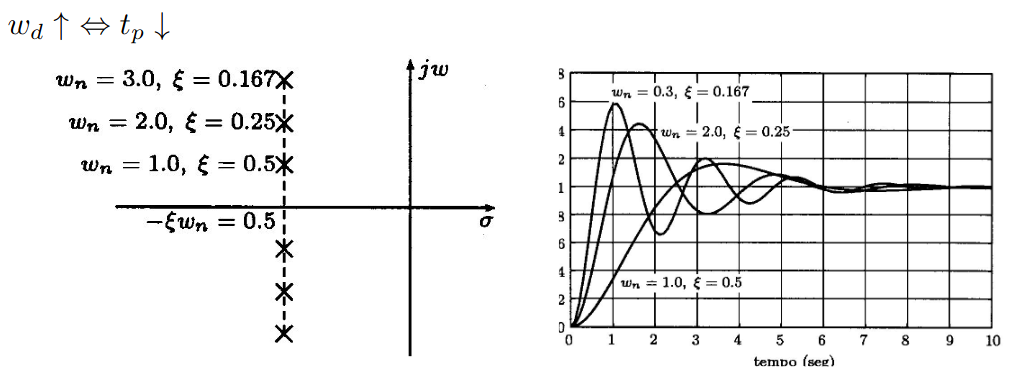
\includegraphics[width=1\textwidth]{img/2/peak-time.png}
            \label{img:peak-t}
        \end{center}
    \end{minipage}
\end{center}

\begin{center}
    \begin{minipage}{0.45\textwidth}
        \begin{itemize}[leftmargin=*]
        \item[] \textbf{\emph{Parâmetro $\mathbf{\sigma}$}}: O parâmetro $w_d$ é constante na continuidade da reta horizontal apresentada. Quanto maior for $\sigma$, menor é o \textit{setting time}.
        \end{itemize}
    \end{minipage}%
    \hfill
    \begin{minipage}{0.55\textwidth}
        \begin{center}
            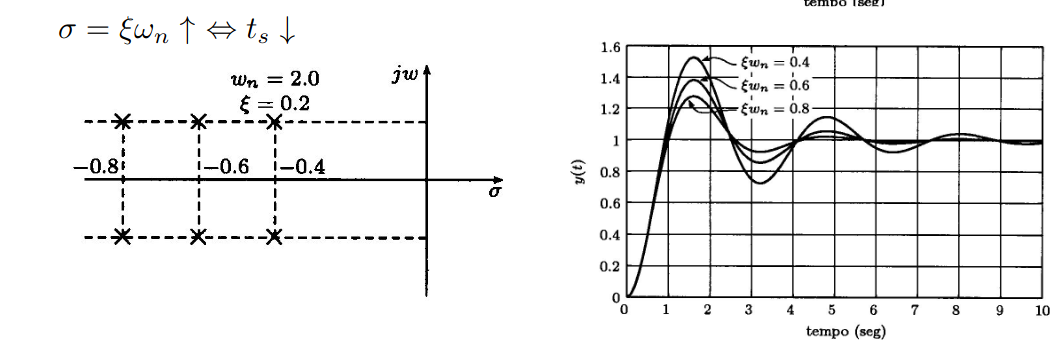
\includegraphics[width=1\textwidth]{img/2/setting-time.png}
            \label{img:set-time}
        \end{center}
    \end{minipage}
\end{center}

%//==============================--@--==============================//%
\newpage
\subsubsection[2.1.3 Influência de pólos e zeros adicionais]{$\pmb{\rightarrow}$ Influência de pólos e zeros adicionais}

\noindent Supondo o seguinte sistema de ordem superior:
$$
    H(s) = \dfrac{25 \cdot a}{(s + a)(s^2 + 4s + 25)}
$$
\noindent  ``The additional pole will contribute more damping to the system response. This will reduce the Percent Overshoot, but at the same time, it will slow the system response increasing Rise Time and Settling Time. Since \textbf{each additional pole contributes an additional exponential term that must die out before the system
reaches its final value}, each additional pole increases the rise time of the system"\cite{FranklinPowell2015} 

\vspace{1 em}
\noindent Quando $|a|$ aumenta
\begin{itemize}
    \item a influência do pólo diminui
    \item O pólo torna-se “menos dominante”
    \item Os pólos complexos tornam-se pólos dominantes
\end{itemize}

\noindent É possível aproximar o sistema de um de segunda ordem (desprezar o pólo não dominante) quando:
\begin{itemize}
    \item Quando o regime transitório associado é desprezável, no conjunto de todas as
contribuições transitórias, ao fim de aproximadamente 5 constantes de tempo.
    \item Quando o módulo do pólo real é pelo menos cinco vezes maior que o módulo
da parte real dos pólos dominantes.
\end{itemize}

\noindent Suponhamos agora os seguinte sistemas:
$$
    \begin{aligned}
        H_1(s) &= \dfrac{2}{(s + 1)(s + 2)} = \dfrac{2}{s + 1} + \dfrac{2}{s + 2}\\[4pt]
        H_2(s) &= \dfrac{2(s + 1.1)}{1.1 (s + 1)(s + 2)} = \dfrac{0.18}{s + 1} + \dfrac{1.64}{s + 2}
    \end{aligned}
$$
\noindent O coeficiente do termo $(s + 1)$ sofreu uma redução drástica com a introdução de um zero na sua periferia (como seria de esperar, se o pólo e o zero possuirem o mesmo termo, a influência do pólo é totalmente anulada). Assim, de forma geral, \textbf{``a zero near a pole reduces the amount of that term in the total response."}\cite{FranklinPowell2015}

\vspace{1 em}
\noindent Neste sentido, a introdução de um zero no semiplano complexo esquerdo (spce) torna o sistema mais rápido (diminuição do tempo de estabelecimento e \textit{rise time}) e aumenta a sobreelevação. Na mesma sequência, a introdução de um zero no semiplano complexo direito (spcd) torna o sistema mais lento e introduz \textit{undershoot} (já que o termo derivativo da resposta no tempo passa a ser subtraído). Sistemas como estes denominam-se \textbf{sistemas de fase não mínima}:

$$
    H(s) = \dfrac{s - 1}{s^2 + s + 1} 
$$

\newpage
{
\mdfsetup{linewidth=2pt}

\begin{mdframed}
    \noindent\textbf{Resumo:}
    \begin{itemize}
        \item Adding a LHP zero to the transfer function makes the step response faster (decreases the rise time
and the peak time) and increases the overshoot.
        \item Adding a RHP zero to the transfer function makes the step response slower, and can make the
response undershoot.
        \item Adding a LHP pole to the transfer function makes the step response slower.
    \end{itemize}

    \noindent Aproximação por sistemas de ordem mais baixa:
    \begin{itemize}
        \item A resíduo associado ao pólo é pequeno (está próximo de um zero) $\rightarrow$ despreza-se o pólo e o zero.
        \item A parte real do pólo é elevada (e portanto possui um regime transitório desprezável) $\rightarrow$ despreza-se o pólo.
    \end{itemize}

    \noindent\textbf{Nota:} O sistema original e o aproximado devem ter o mesmo ganho estático
\end{mdframed}
}

%//==============================--@--==============================//%